\documentclass[a4paper,11pt]{article}

\usepackage[utf8]{inputenc}
\usepackage[a4paper, left=3cm, right=3cm, top=3cm, bottom=3cm]{geometry}
\usepackage[frenchb]{babel}
\usepackage{default}
\usepackage{pslatex}
\usepackage{graphicx}
\usepackage{algorithmic}
\usepackage{multicol}
\usepackage{amsmath}
\usepackage{amssymb}
\usepackage{textcomp}
\usepackage{pgf}
\usepackage{tikz}
\usepackage{pgfplots}
\usepackage{capt-of}
\usepackage{esvect}

\usetikzlibrary{arrows}
\pagestyle{empty}
\definecolor{qqwuqq}{rgb}{0,0.39,0}
\definecolor{xdxdff}{rgb}{0.49,0.49,1}
\definecolor{uququq}{rgb}{0.25,0.25,0.25}
\setcounter{tocdepth}{4}

\renewcommand{\algorithmicwhile}{\textbf{Tant que}}
\renewcommand{\algorithmicendwhile}{\textbf{Fin Tant que}}
\renewcommand{\algorithmicfor}{\textbf{Pour}}
\renewcommand{\algorithmicendfor}{\textbf{Fin Pour}}
\renewcommand{\algorithmicdo}{\textbf{Faire}}
\renewcommand{\algorithmicif}{\textbf{Si}}
\renewcommand{\algorithmicelse}{\textbf{Sinon}}
\renewcommand{\algorithmicendif}{\textbf{Fin Si}}
\renewcommand{\algorithmicthen}{\textbf{Alors}}
\renewcommand{\algorithmicreturn}{\textbf{Retourner}}

% \setcounter{tocdepth}{4}

%opening
\title{Comment simuler numériquement la géomorphologie alpine~?}
\author{Manceau Thibaut, Gros Alexis, Porteries Tristan}

\begin{document}

\maketitle

\clearpage

\tableofcontents

\clearpage

\section{Glossaire}

\subsection{Glossaire géomorphologique}

\begin{itemize}
  \item Géomorphologie~: Science de l'étude des causes de l'apparence des formes qu'étudie la géologie ;
  \item Moho~: Limite entre la lithosphère et l'asthénosphère ;
  \item Orogénèse~: Désigne tous les mécanismes relatifs à la surrection d'un massif montagneux ;
  \item Viscosité~: Plus un fluide est visqueux, plus il s'écoulera lentement.
  Toute roche peut être considérée comme un fluide très visqueux si l'on considère une grande échelle de temps.
\end{itemize}

\subsection{Glossaire informatique}

\begin{itemize}
  \item Boxel~: Matérialisation d'un voxel en tant que cube ;
  \item Étape complète de simulation~: Étape comprenant la résolution de toutes les collisions et cellules ;
  \item Voxel~: Point dans un environnement 3D discret.
\end{itemize}

\section{Introduction}

Cela fait à peine 50 ans que la communauté scientifique a adopté la tectonique des plaques, et malgré de nombreuses recherches, la géologie, discipline encore relativement fragmentaire, est une science assez jeune comparée à la physique et aux mathématiques et qui connaît encore de nombreux points sombres, ignorant toujours la structure profonde de notre manteau. \\
Cependant, nous (Alexis Gros, Tristan Porteries et Thibaut Manceau) pensons qu'il serait intéressant de faire l'état de l'art en ce qui concerne la simulation d'un paysage géomorphologique de façon réaliste.
En effet, cette simulation pourrait grandement aider à l'obtention de nouvelles connaissances sur la géomorphologie, sans compter tous les autres débouchés où elle pourrait remplacer des générateurs de terrains souvent trop peu réalistes. \\
Vous serez ainsi informés dans le présent document de la synthèse de nos recherches sur ce sujet aussi vaste que passionnant, nous ayant donné l'occasion de balayer de nombreux champs de la sciences tels que la chimie moléculaire, la mécanique des fluides ou encore le magnétisme.

\section{Les principes géomorphologiques}

\subsection{Le relief}

Ce que nous appelons « relief » correspond à l'ensemble des formes créés par des processus.
Ces processus sont regroupés sous le nom de « Morphogenèse ».
Nous pouvons les séparer en deux parties~:
\begin{itemize}
  \item les facteurs endogènes, qui correspondent à la formation du paysage (par exemple, la tectonique des plaques)~;
  \item les facteurs exogènes, qui correspondent à la destruction du paysage~: l'érosion\ldots
\end{itemize}
L'homme est également considéré comme un facteur géomorphologique, mais il est à la fois endogène et exogène. \\

Quatre étapes principales composent ces processus~:
\begin{itemize}
  \item l'altération ;
  \item l'érosion ;
  \item le transport ;
  \item la sédimentation.
\end{itemize}
Les débris de roche résultant de phénomènes exogènes sont nommés des altérites. \\
L'altération correspond à tout ce qui modifie les propriétés des roches, ce qui conduit à une destruction partielle ou totale de celles-ci. \\
L'érosion correspond au processus de dégradation et de transformation du relief qui est causé par tout agent externe. \\
Le transport est l'acheminement des altérites par des agents de transport (souvent les mêmes que les agents externes qui réalisent l'érosion). \\
La sédimentation correspond au dépôt des altérites. \\

Les échelles d'espace ne sont pas les mêmes~: l'altération chimique s'étudie a plus petite échelle que l'altération physique~; mais ces deux catégories restent assez ciblées.
L'érosion, le transport et la sédimentation se constatent, pour leur part, à l'échelle du paysage. \\

\subsection{L'altération}
\subsubsection{L'altération physique}

L'altération physique est l'ensemble des altérations qui agissent physiquement sur divers matériaux entre eux~:
\begin{itemize}
  \item la cryoclastie~: Lorsqu'une roche poreuse se remplit d'eau et que cette eau gèle, son volume augmente d'environ 10\%, ce qui provoque des fissures.
  Nous appelons le facteur déterminant la « Gélivité », et elle dépend de la porosité et du taux de fissure de la roche~;

  \medbreak
  \begin{center}
    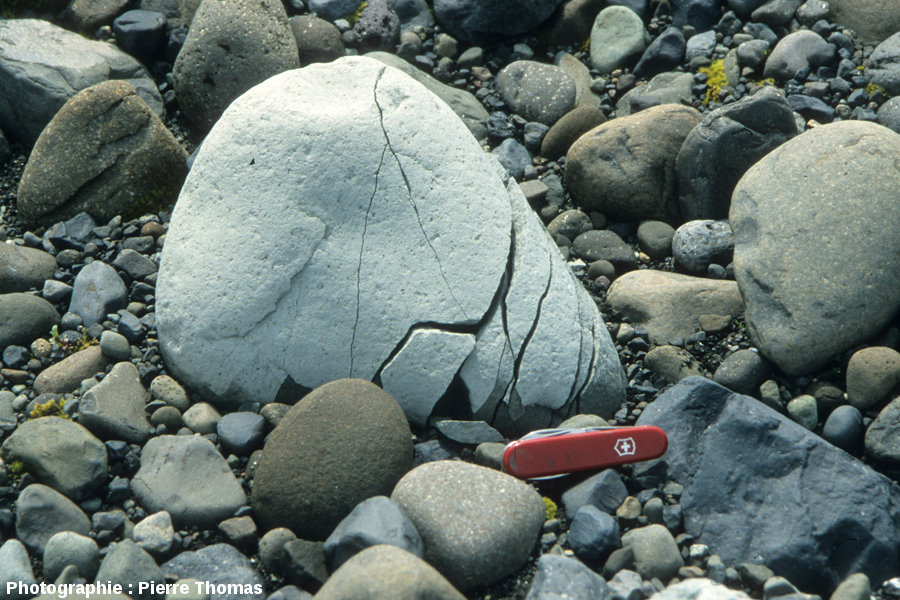
\includegraphics[width=8cm]{Images/Erosion/cryoclastie.jpg}
  \end{center}
  \captionof{figure}{Rocher soumis à une altération de type cryoclastique}
  \medbreak

  \item la thermoclastie~: Processus de fracturation lié aux changements importants et fréquents de variation de température~;
  \item la desquamation~: C'est un enlèvement de lames de roche en pelure d'oignon~;

  \medbreak
  \begin{center}
    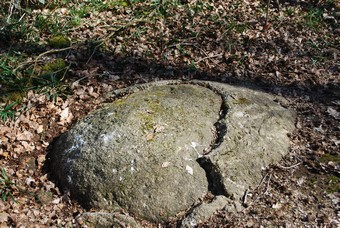
\includegraphics[width=8cm]{Images/Erosion/desquamation.jpg}
  \end{center}
  \captionof{figure}{Faille en « pelure d'oignon » typique d'un enlèvement de matière en desquamation}
  \medbreak
  
  \item l'hydroclastie~: C'est un processus de fracturation lié aux changements de la teneur en eau de la roche. L'eau provoque également un gonflement de l'argile et augmente la pression hydrostatique.
  Lorsque l'eau s'évapore, elle provoque une fracturation par dessiccation (qui correspond au phénomène de desquamation, mais avec des formes s'organisant en réseau de fentes) ;
  \item l'haloclastie~: Elle est due aux cristaux de sel laissés par de l'eau qui s'est évaporée. Ces cristaux de sels vont alors creuser la roche, et ainsi potentiellement la fragmenter.

  \medbreak
  \begin{center}
    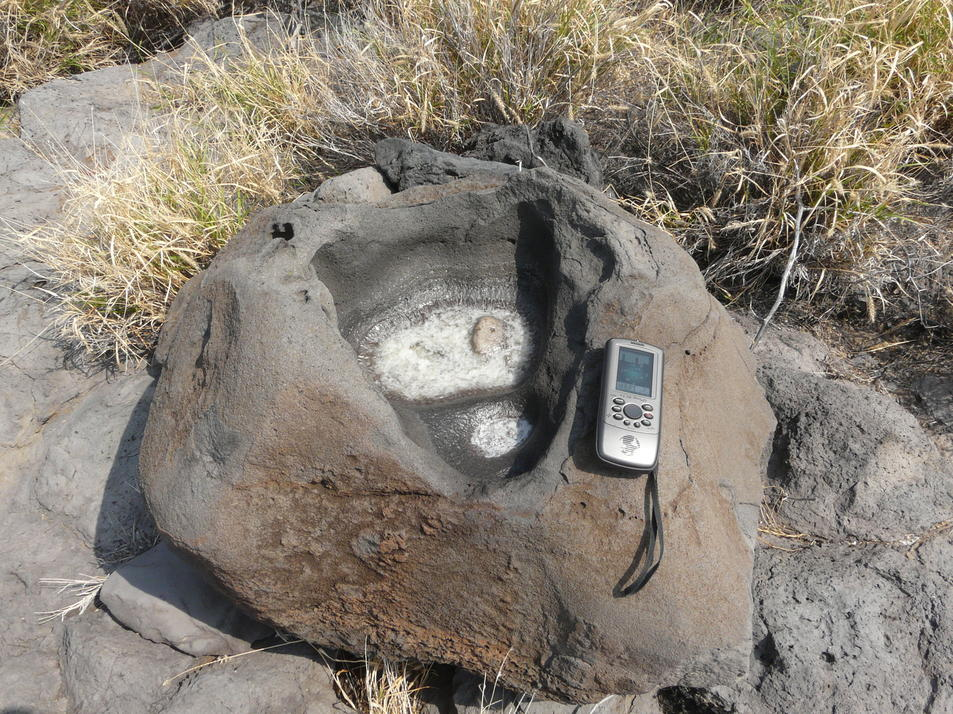
\includegraphics[width=8cm]{Images/Erosion/Haloclastie_vasque_basalte_Hawaii.jpg}
  \end{center}
  \captionof{figure}{Roche creusée par le sel}
  \medbreak

\end{itemize}

\subsubsection{L'altération biologique}

L'altération biologique comprend tout les phénomènes imputables aux êtres vivants. \\
La respiration cellulaire~: qu'elle soit complète ou incomplète, elle entraîne une production de $CO_2$ et d'eau qui influenceront le sol.
Par exemple, la combinaison d'eau avec le $CO_2$ forme de l'eau carbonée qui va solubiliser la calcite.

\begin{center}
  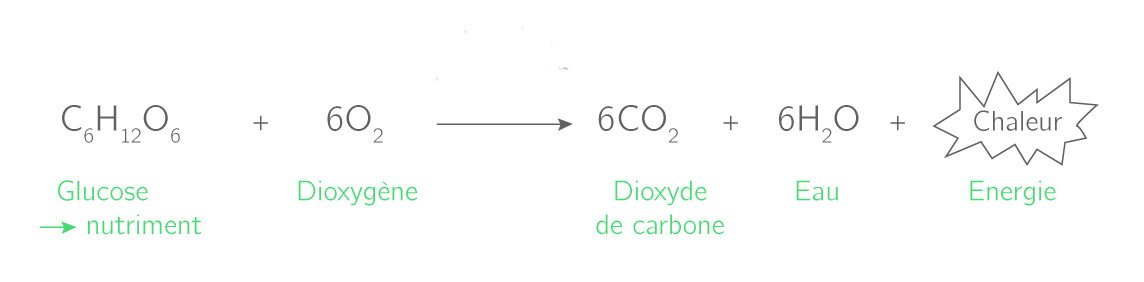
\includegraphics[width=12cm]{Images/Erosion/Respiration_cellulaire.png}
\end{center}
\captionof{figure}{Schéma de la respiration cellulaire}

\subsubsection{L'altération chimique}
\begin{itemize}
  \item mise en solution~: C'est basiquement la réaction d'une roche avec de l'acide ou de l'eau, qui va désagréger celle-ci.
  Par exemple, la réaction de l'eau avec la calcite~:
  \medbreak
  \begin{center}
    \boxed{H_2O + CaCO_3 \Longrightarrow Ca^+ + 2H + CO_3^-} % #inco
  \end{center}
  \medbreak
  \item hydratation et déshydratation, ce qui signifie souvent~: minéral + eau = nouveau minéral hydraté; la déshydratation étant le processus inverse.
  Les réactions les plus importantes sont~:
  \begin{itemize}
    \item la déshydratation du gypse pour produire de l'anhydrite~:
    \medbreak
    \begin{center}
      \boxed{CaSO_4 + 2H_2O \Longrightarrow CaSO_4 + 2H_2O}
    \end{center}
    \medbreak
    \item l'hydratation de l'hématite pour produire de la limonite~:
    \medbreak
    \begin{center}
      \boxed{Fe2O_3 + 3H_2O \Longrightarrow 2Fe(OH)_3} % #inco
    \end{center}
    \medbreak
    \item l'hydratation de la kaolinite pour produire de la gibbsite ;
  \end{itemize}

  \item hydrolyse~: C'est un processus au cours duquel un cation (ion positif) d'un minéral va remplacer un cation $H^+$ d'une solution acide.
  Cette réaction a pour conséquence de détruire le minéral (mise en solution complète) ou de le convertir en une nouvelle espèce (que l'on appellera alors un néo-matériau) ;
  \medbreak
  \begin{center}
    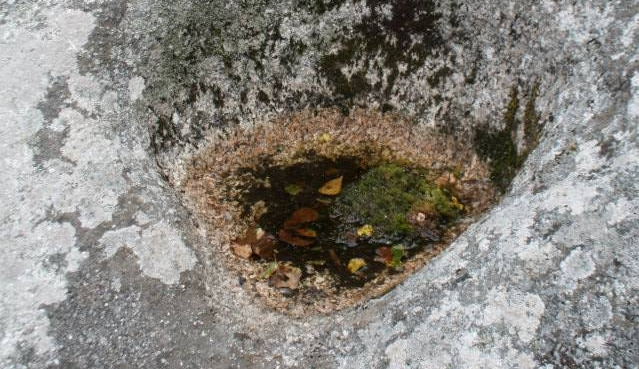
\includegraphics[width=8cm]{Images/Erosion/hydrolyse.jpg}
  \end{center}
  \captionof{figure}{Phénomène d'hydrolyse appliqué à une roche (on le voit à la couleur différente de la roche)}
  \medbreak
  \item oxydation~: C'est la combinaison de métaux (comme le fer et le manganèse) avec l'eau qui provoque une modification de la structure cristalline du minéral ;
  \item dissolution~: désagrègement des molécules en anions et cations par un solvant et dispersion dans l'eau.
\end{itemize}

\subsection{L'érosion}

Nous caractérisons le potentiel d'érosion à partir de deux critères~:
\begin{itemize}
  \item l'érodibilité, qui correspond à la sensibilité du sol à l'érosion ;
  \item l'érosivité, qui correspond à l'intensité potentielle de l'érosion.
\end{itemize}

\subsubsection{L'érosion éolienne}

Le vent est un agent efficace uniquement dans les régions arides car la présence d'une couverture végétale diminue fortement son effet.
Il ne peut déplacer que des éléments fins (les limons sont entraînés à partir d'une vitesse de 3 m/s, les sables nécessitent, pour leur part, 10 m/s).

\begin{center}
  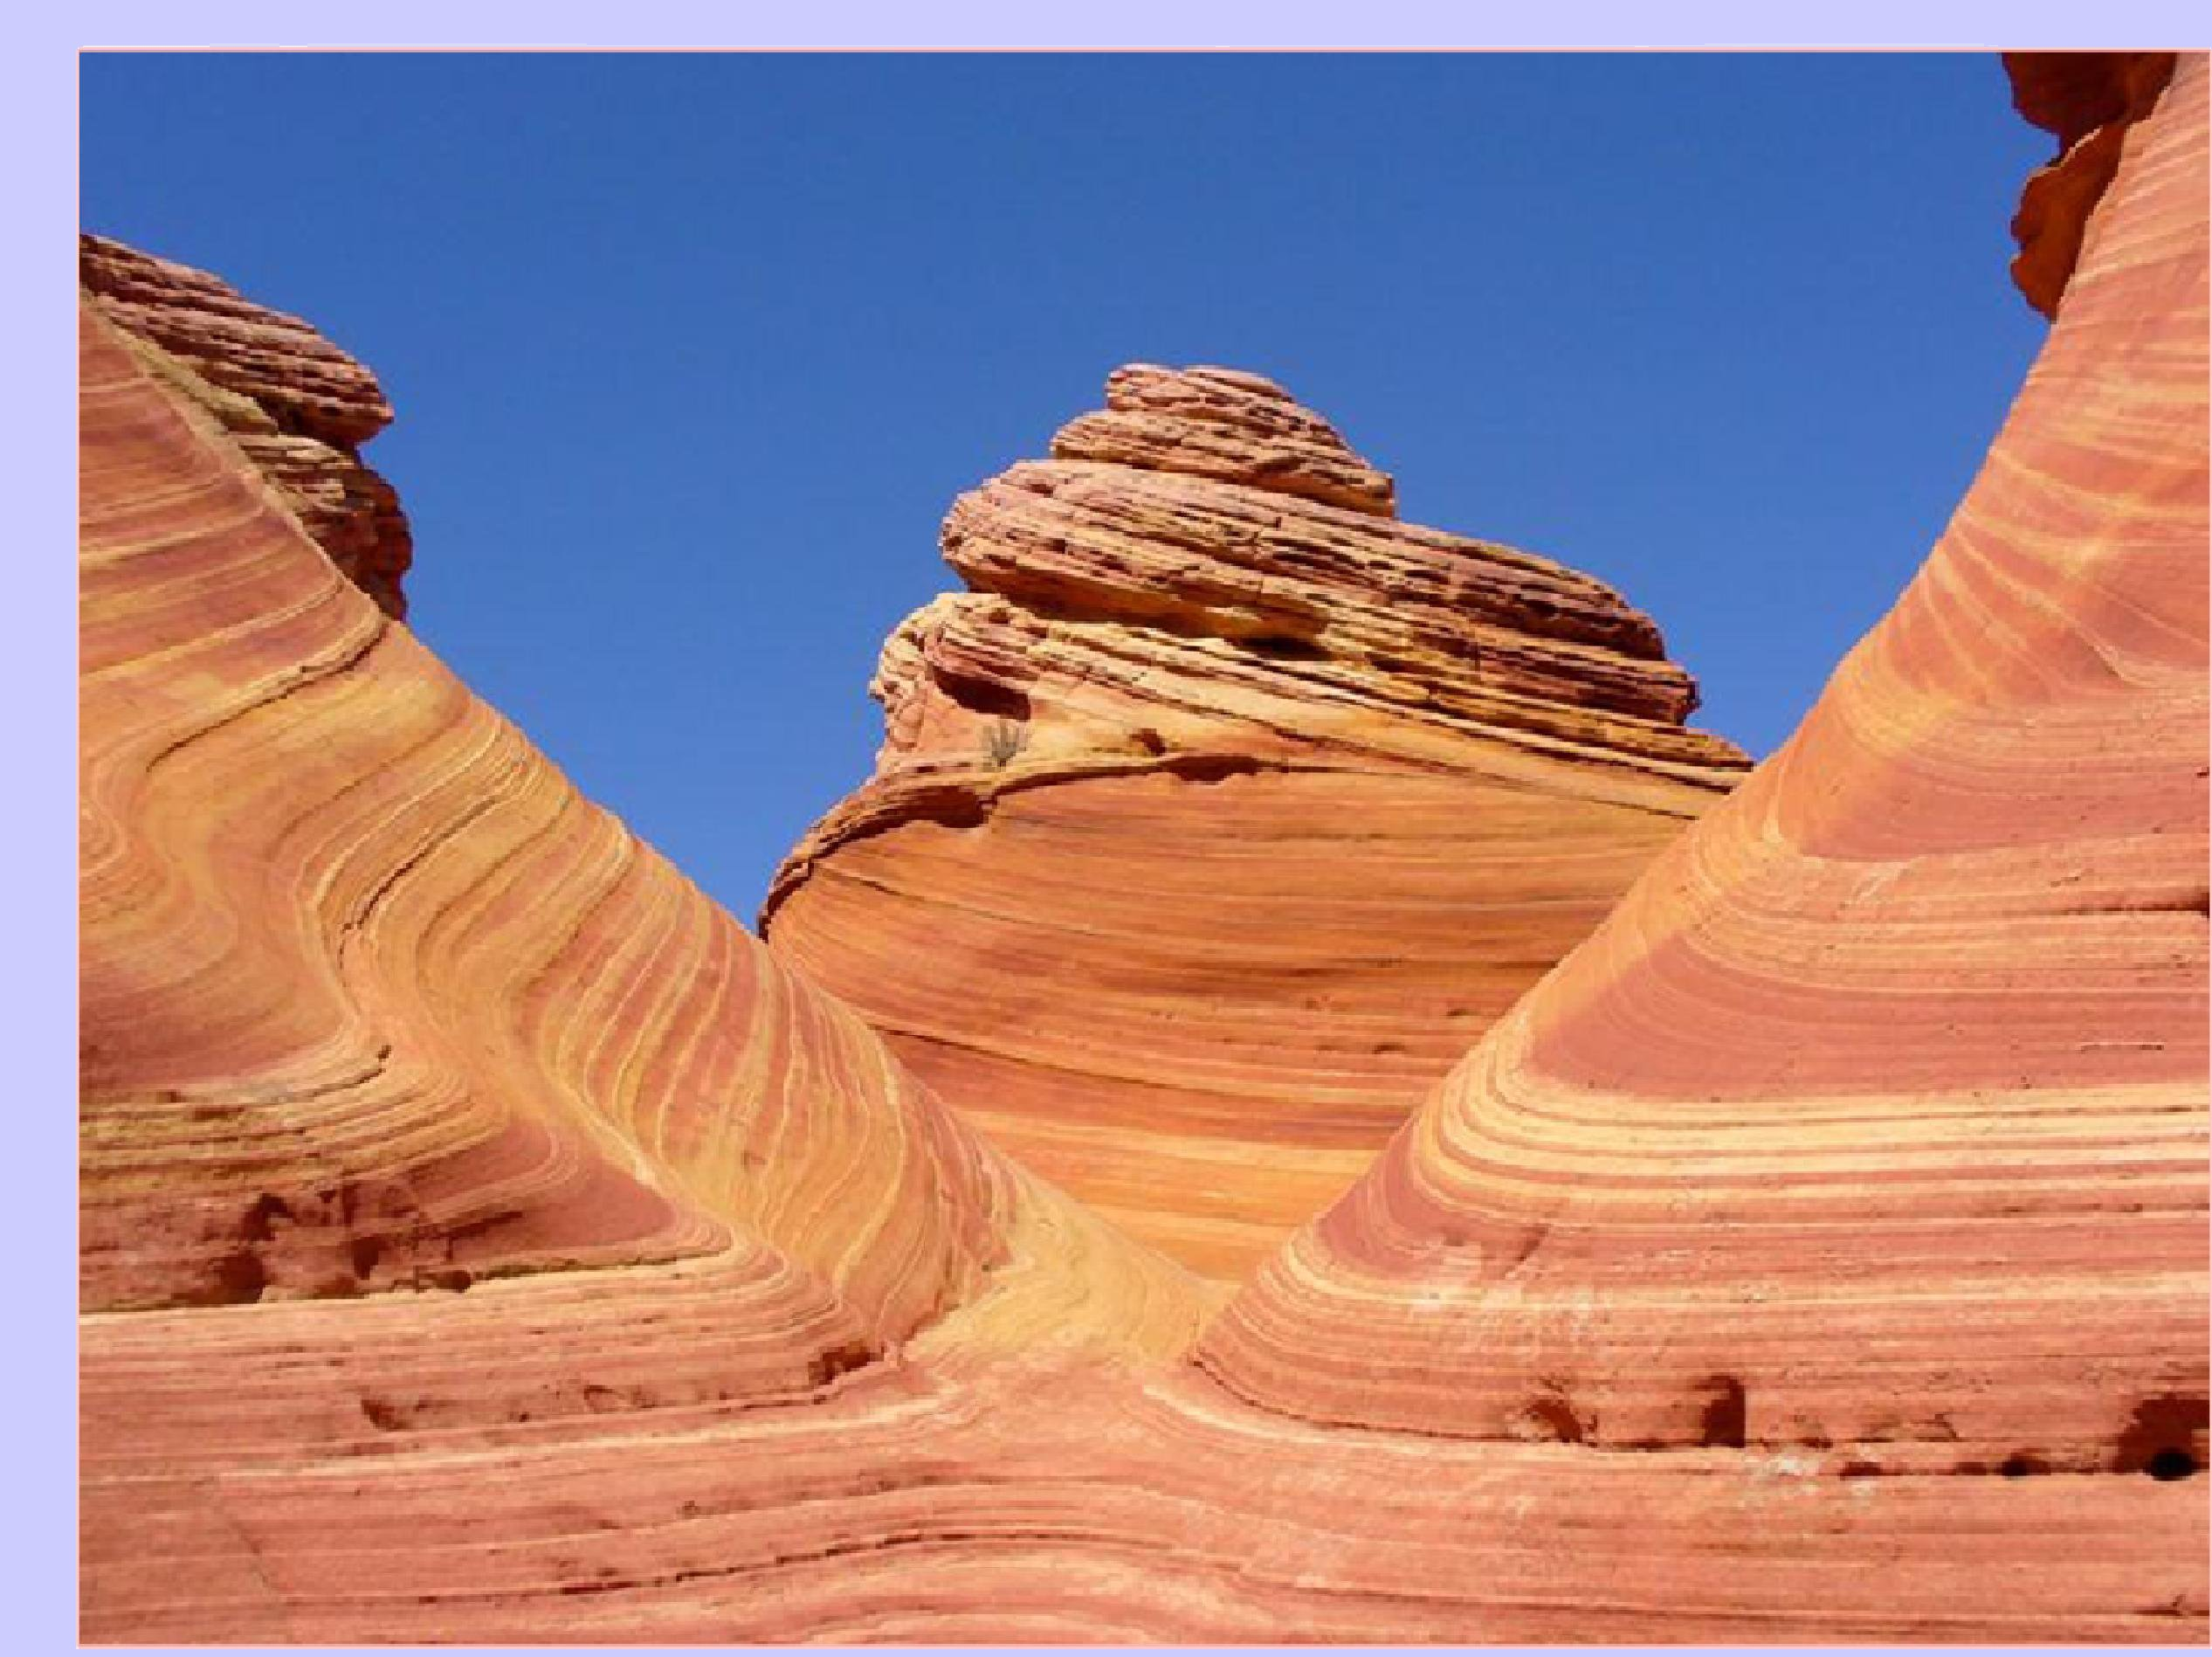
\includegraphics[width=8cm]{Images/Erosion/erosion_eolienne.JPG}
\end{center}
\captionof{figure}{Exemple d'érosion éolienne}

\subsubsection{L'érosion fluviale et le ruissellement}

\paragraph{Le ruissellement}
\medbreak
Le ruissellement se déclenche si les précipitations sont supérieures à la capacité d'infiltration du sol. C'est le cas général des terrains imperméables. 
Après une forte pluie, les eaux empruntent les fissures du sol (à la surface), les élargissent progressivement en chenaux parallèles qui, par la suite, fusionnent avec l'écoulement des arêtes.

\begin{center}
  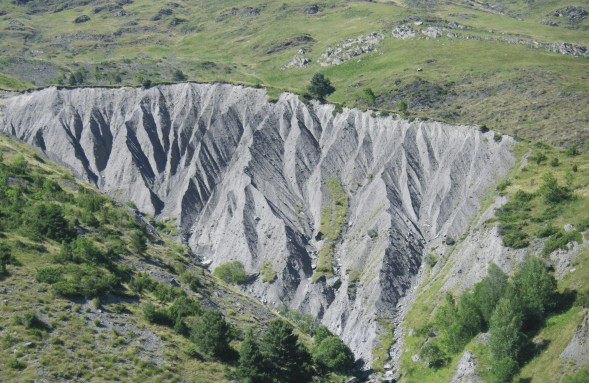
\includegraphics[width=8cm]{Images/Erosion/bad_lands.jpg}
\end{center}
\captionof{figure}{Les « Bad Lands » (ici, en PACA) : exemple d'érosion due au ruissellement}

\paragraph{Les torrents}
\medbreak
Les torrents sont situés en amont des montagnes.
Ils sont décomposables en 3 parties~:
\begin{itemize}
  \item un bassin de réception, où l'eau emporte les différentes roches ;
  \item un chenal d'écoulement, qui est souvent étroit, à forte pente et à fort courant ;
  \item un cône de déjection, où s'amoncellent une partie des altérites.
\end{itemize}

\begin{center}
  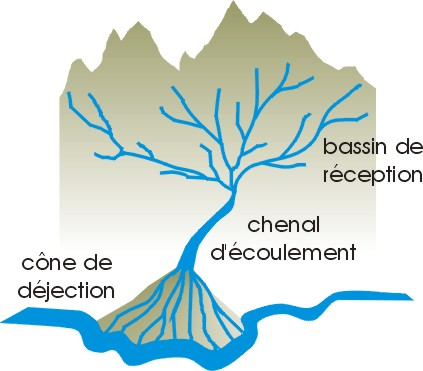
\includegraphics[width=8cm]{Images/Erosion/torrent2.jpg}
\end{center}
\captionof{figure}{Schéma des trois composantes d'un torrent}

\subsubsection{L'érosion karstique}

Toutes les formes d'érosions relatives à la dissolution des roches par de l'eau douce portent le nom de morphologie karstique.
Nous distinguons deux types de morphologie karstique~:
\begin{itemize}
  \item La morphologie souterraine, aussi appelée endokarst.
  Elle est constituée de nombreuses failles et diaclases (pierres fendues mais ne s'écartant pas).
  Nous distinguons deux parties~: la partie active, où s'écoulent les rivières souterraines et la partie fossile, sans eau.
  Nous retrouvons de nombreux attributs qui lui sont propres, comme la présence de stalactites (caractérisées par un canal central où s'écoule l'eau), de stalagmites (pleines), de draperies\ldots
  Toutes ces concrétions résultent du dégazage du $CO_2$, qui provoque la précipitation de $CaCO_3$ ;

  \item La morphologie aérienne, aussi appelée exokarst.
  Nous pouvons citer les dollines, de grandes dépressions qui proviennent de l'agrandissement de failles dues à l'infiltration de l'eau~; les canyons, où encore les rivières sèches (toute l'eau ayant été absorbée par le sol).
\end{itemize}

\begin{center}
  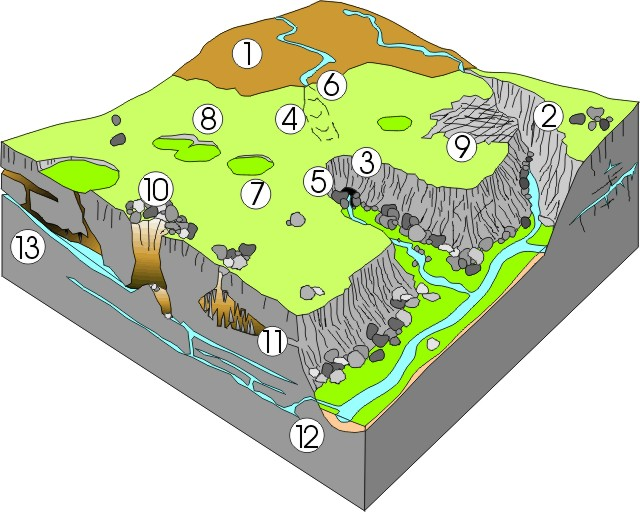
\includegraphics[width=8cm]{Images/Erosion/karst_new_col.jpg}
\end{center}
\captionof{figure}{Schéma des différentes morphologies karstiques}

\subsubsection{L'érosion glaciaire}

L'érosion glaciaire dépend de la température de la base du glacier~:
Si la température est assez élevée, un fin film d'eau se forme et entraîne le glacier vers le bas de la vallée. Au contact de cette grosse masse d'eau, les débris s'incorporent à la glace et sont emportés.
Si la base du glacier est froide, celui-ci ne se déplace que par déformation plastique et l'érosion est minimale.
A grande échelle, nous pouvons observer des vallées qui peuvent être à faible pente (correspondant à un élargissement du glacier) ou à forte pente (correspondant à un rétrécissement).
Lorsque deux ou plusieurs glaciations se sont succédées, nous pouvons observer des vallées avec plusieurs auges. 
A petite échelle, l'érosion glaciaire se manifeste par des surfaces polies et souvent striées à cause du poids conséquent du glacier (des stries glaciaires).
Dans beaucoup de cas, ces roches présentent une pente plus faible vers l'amont (usure) que vers l'aval (arrachement de blocs), ce qui permet de reconstituer le sens d'écoulement des glaciers.

\begin{center}
  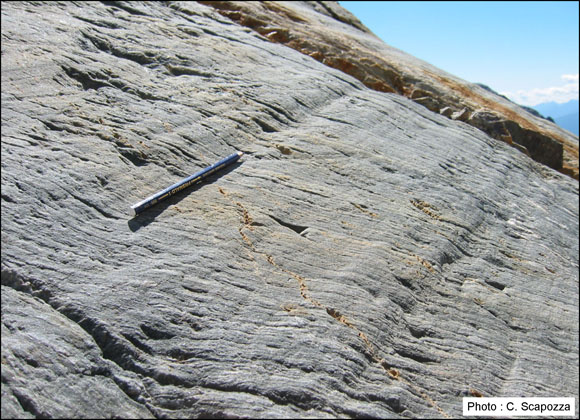
\includegraphics[width=8cm]{Images/Erosion/stries_glaciaires.jpg}
\end{center}
\captionof{figure}{Photo de stries glaciaires}

\subsubsection{L'érosion marine}

Les principaux agents de l'érosion marine sont les vagues et les courants, auxquels on peut ajouter l'action du sel emportés par le vent (processus d'haloclastie due à la cristallisation de sel dans la porosité et les fractures.
Les vagues ont un pouvoir érosif dû à plusieurs facteurs~:
\begin{itemize}
  \item un mitraillage de la surface par les débris (gravier et sable) transportés ;
  \item une force de succions lorsqu'elles se retirent ;
  \item des vibrations pas suite de chocs successifs.
\end{itemize}
Les altérites sont ensuite séparés selon leur poids~: les plus fins restent en suspension alors que les plus gros se déposent au fond.
Les grains de sable qui subissent l'action des vagues ont un aspect émoussé-luisant, contrairement à ceux transportés par le vent qui ont un aspect rond-mat. \\

L'érosion des façades littorales par la mer se produit par sapement et éboulement (l'eau creuse le bas de la falaise, ce qui provoque l'effondrement du mur).
Nous distinguons les falaises vives (encore érodées par les vagues) des falaises mortes (séparées par un banc de sable de la mer).

\begin{center}
  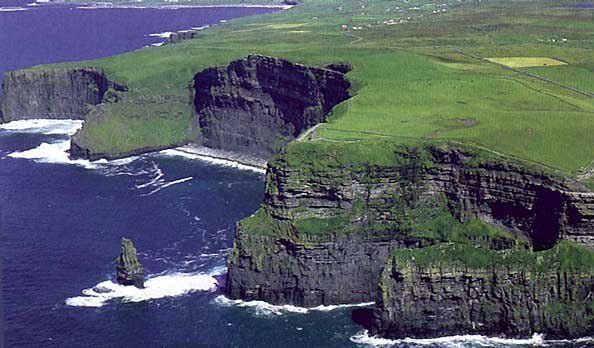
\includegraphics[width=8cm]{Images/Erosion/cliffs.jpg}
\end{center}
\captionof{figure}{Photo d'une facade marine}

\subsection{Le transport}
Il existe trois types de transport~:
\begin{itemize}
 \item le glissement de masse (sans fluides) ;
 \item les écoulements gravitaires (avec fluides) ;
 \item les écoulements d'eau, d'air ou de glace.
\end{itemize}

\subsubsection{Le glissement de masse}

Ils se produisent lorsque la pente est raide.
Le déplacement est court (de l'ordre du kilomètre) mais la quantité de matière transportée peut être très importante.
Le déplacement provient d'une fissure avec la masse rocheuse qui délie la surface rocheuse.
Les fluides n'ont aucun impact sur ce type de transport (sauf si nous considérons qu'ils sont la cause de la fissure).

\subsubsection{Les écoulements gravitaires}

Ils proviennent de la mise en solution d'altérites~; toutefois, nous les distinguons des écoulements de fluides simples car c'est la gravité qui provoque leur déplacement. Les pentes soumises à ce type de transport sont faibles.

\subsubsection{L'écoulement d'un fluide}

C'est le fluide qui est responsable du déplacement.
Sa capacité à transporter des altérites dépend de nombreux facteurs, dont sa masse volumique, sa vitesse et sa viscosité.
Les différences entre l'air, l'eau liquide et les glaciers provient de cette différence de masse et de viscosité.
La vitesse du fluide permet de distinguer deux types d'écoulement~: laminaire et turbulent.
Un écoulement laminaire peut être qualifié de « tranquille »~: les filets d'eau restent parallèles entre eux.
Un écoulement turbulent, pour sa part, voit ses filets d'eau partir dans tous les sens~: le transport est conditionné par les altérites qu'il transporte.
C'est le « nombre de Reynolds » (Re) qui permet de distinguer si un écoulement est laminaire ou turbulent~:
\begin{center}
  \boxed{\displaystyle{Re = \frac{V \times L}{\nu}}}
\end{center}
Où V est la vitesse du fluide (en m/s), $L$ sa viscosité cinématique (en $m^2/s$) et $\nu$ la dimension caractéristique (en m).

\begin{center}
  \boxed{\displaystyle{\nu = \frac{\mu}{p}}}
\end{center}
Où $p$ est la masse volumique du fluide (en $kg/m^3$), $\mu$ sa viscosité dynamique (en Pa.s).
\medbreak
Si Re est compris entre 500 et 2000, l’écoulement est laminaire.
Les glaciers, de part leur forte viscosité, réalisent un écoulement laminaire.
C'est également le cas des rivières à très faible pente.
Si Re est supérieur à 2000, l’écoulement est turbulent.
C’est le cas de la plupart des rivières et du vent.
Nous distinguons également le courant torrentiel, qui est dû à une très forte vitesse du fluide.
Nous pouvons savoir si un liquide exerce un écoulement torrentiel grâce au « nombre de Froude » (F)~:
\begin{center}
  \boxed{\displaystyle{F = \frac{V}{g \times r} \times \frac{1}{2}}}
\end{center}
où V est la vitesse du fluide, g l'accélération de la pesanteur et r la profondeur du chenal dans lequel se fait l'écoulement.
Si F est supérieur à 1, l’écoulement est torrentiel.
Si F est inférieur à 1, l’écoulement est turbulent. \\

\subsubsection{Le transport des sédiments}

Nous distinguons trois types de transport de sédiments, qui dépendent de la masse des sédiments~:
\begin{itemize}
  \item le roulement, pour les altérites les plus gros ;
  \item la saltation (ou le transport par rebond) pour les éléments de masse moyenne ;
  \item la suspension pour les éléments les plus légers.
\end{itemize}

\begin{center}
  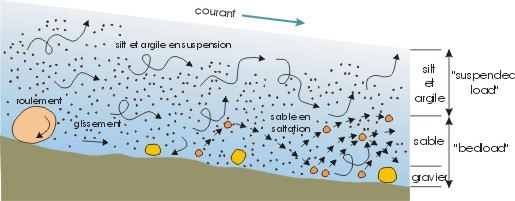
\includegraphics[width=10cm]{Images/transport_0.png}
\end{center}
\captionof{figure}{Schéma du transport de sédiments}

La charge en suspension des écoulements turbulents est beaucoup plus importante que celle des écoulements laminaires.

\subsubsection{Le diagramme de Hjulström}
Ce graphe (essentiellement basé sur des expériences en laboratoire) montre la vitesse minimale d'un courant nécessaire pour mobiliser, transporter et déposer des grains de quartz de granulométrie variable.

\begin{center}
  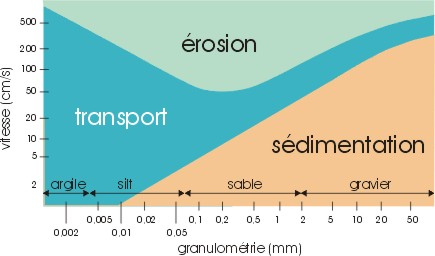
\includegraphics[width=10cm]{Images/transport_1.png}
\end{center}
\captionof{figure}{Diagramme de Hjulström}

\subsection{Le dépôt des sédiments}

Dès qu'une particule est mise en suspension, elle commence aussitôt à sédimenter. Sa vitesse de sédimentation est donnée par la loi de Stokes~:
\begin{center}
  \boxed{v = c \times d2}
\end{center}
Où c est une constante égale à~:
\begin{center}
  \boxed{\displaystyle{(rp -rf) \times \frac{g}{18\mu}}}
\end{center}

Où $v$ représente la vitesse de sédimentation, $\mu$ la viscosité du fluide, $rf$ sa masse volumique et $rp$ celle de la particule; $d$ est le diamètre de la particule.

\subsection{Quelques rappels sur la géologie}

\subsubsection{La tectonique des plaques}

Imaginée par Wagner au $19$ siècle, redécouverte dans les années 50 pour n'être qu'unanimement acceptée dix ans plus tard, la théorie des plaques signe le véritable commencement de la géologie en tant que science, changeant totalement notre vision de la terre et de ses cycles. \\
La tectonique des plaques propose que l'écorce terrestre soit formée de plaques qui se déplaceraient les unes par rapport aux autres à la faveur des mouvements internes du manteau terrestre. Ce même manteau qui, encore de nos jours, reste bien mystérieux (notamment en ce qui concerne les points chauds). \\
\\
La mécanique de la terre, qui est à la source de tous les effets géomorphologiques visibles, est en fait le résultat d'un long refroidissement qui commença il y a 4,6 milliards d'années et qui se poursuit encore aujourd'hui.\\
Cette mécanique de refroidissement met en place d'autres mécanismes comme ceux de la fermeture et de l'ouverture des océans, causes majeures de la plupart des mouvements à la surface de la terre.

\subsection{La subduction}

La subduction désigne la plongée d'une plaque sous une autre (voir figure ci-dessous). Ces plaques sont dites lithosphériques (car possédant une lithosphère, pour simplifier, une partie solide séparée de l'asthénosphère par le moho). Elles sont portées par l'asthénosphère, la partie « manteau » des plaques. \\
Une subduction survient généralement quand une plaque océanique vieillissante plonge sous un continent. En fonction de l'angle d'incidence et de la vitesse de la plaque plongeante, différent types de phénomène orogéniques sont visibles à la surface. Par exemple, des séismes fréquents qui créent une chaîne de montagne. \\
De nos jours, ce phénomène se manifeste encore à grande ampleur dans les Andes, et des traces de subductions se trouvent aux quatre coins du globe, de l'Inde au Japon en passant par les Alpes. \\

\begin{center}
  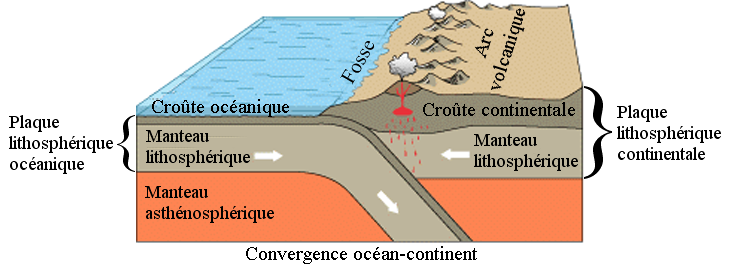
\includegraphics[width=8cm]{Images/subduction_2.png}
\end{center}
\captionof{figure}{Schéma de la subduction entre deux plaques tectoniques.}

\subsubsection{L'histoire de la chaîne alpine}

Le début de l'histoire de la chaîne alpine commence peu après -256 Ma. À cette époque, le paléoocéan Thétys occupait la majorité de la surface terrestre. \\
Les contraintes du manteau terrestre amorcèrent alors le soulèvement d'une zone de la plaque alpine, préfigurant une dorsale océanique.
\begin{itemize}
  \item - 200 Ma, trias~: ouverture de l'océan alpin.\\
  La dorsale est pleinement ouverte et déverse son  magma dans l'océan alpin, ce qui a pour effet de l'élargir.
  A son apogée, l'océan Alpin fut large de 300 à 1000 km, et profond de 3500 à 4000 m ;
  \item - 140 Ma, crétacé inférieur~: début de la compression de l'océan alpin suite à des contraintes externes telles que le rapprochement de la plaque Africaine ;
  \item Fin du crétacé inférieur, subduction du coté de la plaque africaine ;
  \item Nouvelle océanisation dans « la zone valaisaine » (nouvelle dorsale typique des océans en fin de vie) ;
  \item Crétacé supérieur~: fin de l'océan alpin, qui est considérablement réduit, et commencement de la mer alpine, reliée à l'océan atlantique en formation. L'océan valaisin est, pour sa part, totalement refermé ;
  \item -65 Ma, paléocène~: Sous l'effet des contraintes, émersion de la plate-forme continentale au delà de la « zone valaisaine ».
  Début de la formation des alpes avec la poursuite de la compression.
  La zone du massif du mont blanc passe sous la zone d'obduction majoritaire pour ressurgir plus tard à sa place actuelle ;
  \item Oligocène~: Écaillage important des couches ;
  \item - 23 Ma~: néogène, création du jura au devant des alpes par effet collatéral de compression ;
  Soulèvement du massif du Mt Blanc, ce qui pousse la partie calcaire des Alpes à glisser par gravité ;
  \item Pliocène~: séparation de la partie calcaire des alpes et pré-alpes (Jura, Chartreuse, Vercors) du reste, désormais essentiellement granitique). Cette séparation se produit par glissement de la partie supérieur calcaire qui s'éloigne de la zone de surrection du Mont blanc.
  C'est à ce moment qu'est atteint le pic d'intensité dans la formation des alpes.
\end{itemize}
Plus récemment, dans les dernières centaine de milliers d'années, les nombreuses ères glacières successives ont totalement refaçonnées le massif des alpes, et c'est cette époque qui reste malgré son âge assez faible la plus décisive dans le façonnage des massifs alpins.
  Le glacier du Rhône tout particulièrement, assez titanesque, a creusé un immense sillon qui laissera place notamment au Lac Léman. 

\subsection{Dynamique des roches}
	
Les physiciens ont grandement fait avancer la géologie modernes grâce aux roches car la connaissance de la dynamique des roches face à un contexte donné éclaire sur la formation et l'évolution des grands systèmes orogéniques comme des déformations à petite échelle.
En effet, les roches, bien qu'usuellement cassantes et rigides, peuvent devenir plus ductiles sous certaines conditions. \\

\subsubsection{Le temps}

Le temps est l'élément fondamental de la géologie car même les roches les plus dures se déformeront comme de la pâte à modeler si elles sont soumises à une force puissante dans le même sens pendant plusieurs dizaines de milliers d'années. C'est d'ailleurs pour cela qu'on utilise de la pâte à modeler dans les modélisations géologiques à petite échelle.\\
En effet, sur les échelles immenses qui sont celles des temps géologiques, n'importe quel matériau se comportera comme s'il était mou.\\
Par exemple, une montagne, sous certaines conditions, peut se transformer en colline en seulement quelques millions d'années.\\
Autre exemple, la « mort des océans », dûe à la lithosphère océanique qui, étant plus dense que la croûte continentale, se refroidit et s'alourdit lentement au fil des millénaires.\\
Il est avéré qu'à cause de ce principe, la durée de vie des océans est limitée à environ 270 millions d'années.\\
Les océans suivent donc un cycle de naissance, vie et de mort qui est directement à la source de la plupart des mécanismes orogéniques.

\subsubsection{La température}

Plus il fait chaud, plus une roche est fluide.\\
C'est le cas pour toutes les roches ; ainsi, l'aspect « pâte à modeler » des roches est accentué en profondeur par la chaleur qui les rend plus malléables.\\
Cela se ressent sur les séismes~: il existe une limite assez floue mais bien réelle qui sépare les séismes cassants, qui se déplacent brusquement à intervalle régulier, des séismes coulissant, où les roches supportent leur déformation progressive en coulissant entre elles comme des fluides très visqueux.

\subsubsection{La pression}

Un facteur auquel nous pensons rarement en premier mais qui est en réalité tout aussi important que les autres.
En effet, la pression des grandes profondeurs empêche les roches de devenir liquides trop rapidement au fur et à mesure qu'elles s'enfoncent.\\
A l'inverse, une brusque remontée de roche des profondeurs, comme c'est le cas avec les volcans par exemple, les font fondre et augmentent plus encore la pression qu'ils exerçant sur le « toit ».\\
C'est ce qui explique que le magma des volcans remonte jusqu'à une certaine hauteur, s'infiltrant par les failles, puis que c'est alors au tour du gaz de fournir la pression nécessaire à l'expulsion du magma.

\section{La simulation}

\subsection{Modéliser un paysage géologique}

Il y a beaucoup de moyens de simuler certains comportements dynamiques en géologie.\\
La plupart font appel à une expérience physique mais quelques unes, plus ou moins récentes, font exclusivement usage du numérique.\\
Pour rester cohérents avec notre problématique et notre objectif, nous avons choisi cette seconde voie.

\subsubsection{Les simulations physiques}

\paragraph{Simulation par pâtes}
\medbreak
Il est fréquent chez les chercheurs géologues de remplacer les couches par divers ingrédients plus ou moins courants~: de la pâte à modeler, du sable mélangé avec de l'huile ou tout autre pâte ductile colorée.
Ces différentes couches sont soigneusement empilées et leurs propriétés sont choisies avec soin de sorte à faire l'analogie avec les couches géologiques d'un paysage réel.
Ces simulations, bien que limitées, arrivent à représenter des contraintes de déformation très précises, pour avoir un aperçu visuel d'une démonstration en géologie (ex~: tectonique des plaques, démonstration par l'expérience de l'existence de certains types de plissements) ou pour démontrer l'existence de certains comportements et propriétés dans un système géologiques.
La plupart de ces simulations sont utilisées, encore aujourd'hui (par souci de rapidité et de réalisme), et modélisent des phénomènes très précis en utilisant des propriétés physiques.
Ils simulent souvent les phénomènes de compression et donc de plissement par différentes couches successives de pâte à modeler de consistance et de propriété différentes pour simuler les phénomènes observés dans la nature.\\
La collision de la plaque indienne avec la plaque euro-asiatique a ainsi reçu une illustration réaliste grâce à un pressoir en métal (représentant l'inde) s'enfonçant dans de la pâte à modeler (représentant l'Asie).
D'autres simulations du même genre mettent en valeur certains types de plis, plis couchés, plis droits et autre. Cependant, ces différentes simulations, bien que très parlantes, prouvent rarement des conjectures car elles sont difficilement reproductibles et nécessitent surtout beaucoup de suppositions qui détachent leur mises en œuvre de la réalité.

\begin{center}
  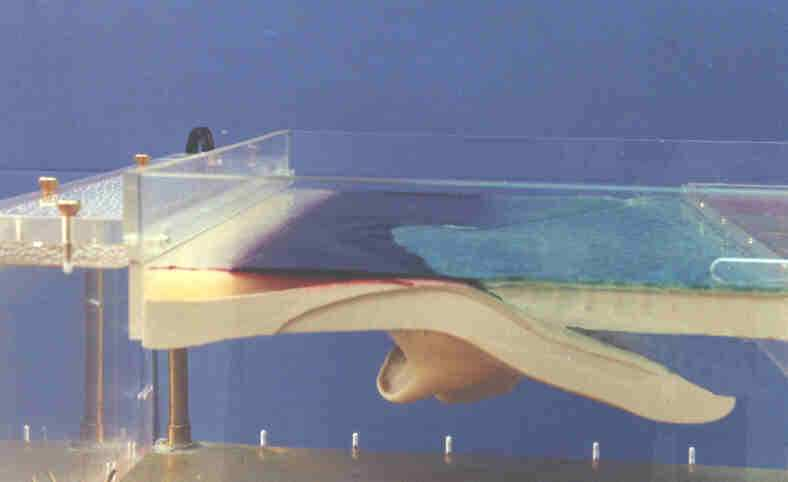
\includegraphics[width=6.2cm]{Images/simulation_physique.png}
  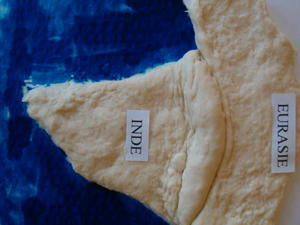
\includegraphics[width=4cm, angle=90]{Images/inde.jpg}
\end{center}
\captionof{figure}{A droite~: Photo de simulation physique par couches de pâtes. A gauche~: Photo de simulation par pâtes des indes.}

\paragraph{La place de la physique dans la simulation}
\medbreak
Dans ce contexte, la géologie a beaucoup appris de la physique, qui l'a amené à conduire d'autres types d'expériences pour trouver les propriétés de certaines roches soumises à des conditions de pressions et de températures intenses, ou bien pour trouver les réactions chimiques opérant lors de l'érosion de roches calcaires par un milieu riche en $CO_2$.

\subsubsection{La simulation numérique par automate cellulaire}

Nous avons épluchés plusieurs thèses traitant de la simulation de phénomènes géologiques grâce aux ordinateurs.\\
Nous n'aurons malheureusement pas trouvé le code source de ces logiciels (ce qui nous aurais permis de les intégrer à notre moteur). De plus, nous avons émis une requête auprès d'un des scientifique ayant basé sa thèse sur une simulation comme la nôtre, mais celui-ci ne nous a pas répondus.\\
Une thèse en particulier a retenu notre attention : elle portait sur la simulation des mouvements de l’asthénosphère et des systèmes de simulation d'érosion.\\
Cette simulation permettait de représenter une subduction grâce à des automates cellulaires. Ces automates étaient représentés grâce à un algorithme se réagençant à chaque pas de la simulation.\\
C'est notamment de là que nous viens l'idée d'avoir utilisé des cellules indépendantes.\\
Cette simulation était assez convaincante visuellement, mais fondamentalement très biaisée car le mouvement des cellules de la première plaque était artificiellement forcé vers le bas pour un meilleur rendu visuel, de sorte que l'apparence primait généralement sur le réalisme physique de la simulation.

\begin{center}
  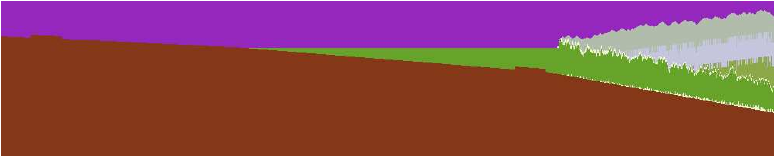
\includegraphics[width=8cm]{Images/3100_cell.png}
\end{center}
\captionof{figure}{Images d'une simulation par automates cellulaire bidimensionnelle à 3100 itérations.}
\begin{center}
  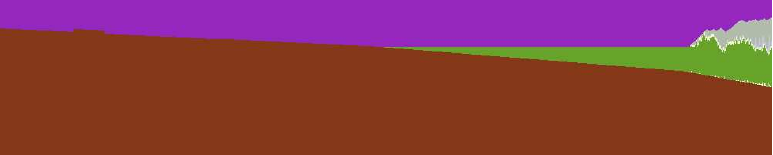
\includegraphics[width=8cm]{Images/7100_cell.png}
\end{center}
\captionof{figure}{Images d'une simulation par automates cellulaire bidimensionnelle à 7100 itérations.}

\paragraph{Simulation par voxels}
\medbreak
La simulation par voxels, particulièrement utile pour l'érosion, consiste à créer un terrain exclusivement composé de « cubes », de points alignés sur un quadrillage en deux ou trois dimensions de coordonnées discrètes.\\
Habituellement, les données de traitement numérique de rendu utilisent des points, reliés entre eux par des traits formant des triangles, qui sont ensuite utilisés pour rendre les formes en perspectives.\\
Les voxels, eux, créent des terrains uniquement composés de cubes, les boxels (voir Glossaire) de sorte qu'ils remplissent l'espace autour d'eux de la largeur d'une unité du système discret.\\
Ce système est avantageux quand on regarde le matériel : le processeur d'un ordinateur ayant du mal avec les nombres à virgule, les voxels lui simplifient grandement la tâche.\\
En effet, il devient bien plus rapide d'effectuer des opérations simples comme rechercher une cellule adjacente dans le maillage, en supprimer ou encore d'optimiser l'affichage en fonction de la présence ou non de cellules adjacentes.\\
De plus, ce système offre l'avantage de permettre de changer assez facilement la résolution des boxels.
En effet, on peut les simplifier à l'affichage en les rendant plus gros, ce qui allège la tâche de la carte graphique.\\
De plus, de la même façon que dans les images en deux dimensions la plus petite unité considérée est le pixel, le boxel est son équivalent en 3D, ce qui implique que les algorithmes de compression classiques des images 2D (type png, jpeg, gif) peuvent s'appliquer sur des portions ou la totalité d'un terrain ainsi généré (moyennant des modifications mineurs), ce qui permet une économie de mémoire énorme.\\
C'est pour toutes ces raisons qu'un modèle d'érosion intelligent basé sur un automate cellulaire 3D permettrait de simuler avec une grande précision un paysage de type alpin, tout en économisant beaucoup de mémoire (moyennant quelques optimisations).

\subsection{Les Cellules}
\subsubsection{Définition d'une cellule}

Premièrement, nous devons définir le plus petit élément de cette simulation. On appellera cet élément une cellule.\\
Une cellule est un morceau de terrain sphérique ou cubique d'environs 10 mètres. Cette taille peut varier mais n'a aucune importance dans la simulation car nous pouvons dire que tout est relatif.\\
Elle est le seul élément incompressible mais les liens entre les cellules sont compressibles.
Une cellule a pour caractéristiques immuables~:
\begin{itemize}
  \item son type de roche~: des caractéristiques propres au type de roche seront utilisées pour les calculs de compression et de friction~;
  \item sa plaque tectonique~: le seul moyen pour la différencier des autres cellules lors d'une collision de plaques.
\end{itemize}
Et comme caractéristiques mutables~:
\begin{itemize}
  \item sa position~: la position de la cellule dans un ensemble non discret ;
  \item sa vélocité~: le vecteur vitesse de la cellule équivalent au déplacement qu'effectuera cette cellule à la fin d'une étape complète de simulation.
\end{itemize}

Si nous prenons toutes les cellules de surfaces et formons des triangles entre elles, nous pourrons alors obtenir une visualisation graphique de la surface du terrain se déformant.

\subsubsection{Disposition des cellules}

Les cellules étant le plus petit élément composant le terrain, leur organisation importe tout particulièrement au début de la simulation.\\
Plusieurs dispositions ont été essayé avant d'arriver à celle utilisée actuellement.\\
Pour simplifier la programmation, les cellules ne sont disposées que sur un plan pour permettre l'utilisation d'un modèle deux dimensions, qui se révèle bien plus simple à écrire et à déboguer. Ainsi, nous gardons des vélocités strictement en deux dimensions. Toutefois, nous utiliserons des vecteurs en trois dimensions (pour permettre une évolution sans avoir à réécrire le code).  \\
Après avoir choisi un modèle cellulaire planaire, nous devions choisir comment organiser ces cellules les unes par rapport aux autres.\\
Toutes les modèles de disposition ont plusieurs points communs~: lors de la création des cellules, la disposition devra créer jusqu'à $n_x$ cellules en abscisse et $n_y$ en ordonnée.
La première disposition choisie fut une grille carré, avec une grille nous faisons simplement une itération $x$ à $x_n$ et imbriqué à l'intérieur une autre itération de $y$ à $y_n$.

\medbreak
\begin{algorithmic}[1]
    \FOR{$x$ de $0$ jusqu'à $(x_n - 1)$}
      \FOR{$y$ de $0$ jusqu'à $(y_n - 1)$}
	\STATE Créer une cellule à la position $(x, y)$.
      \ENDFOR
    \ENDFOR
\end{algorithmic}
\medbreak

L'avantage de cette méthode était sa simplicité, mais l'inconvénient d'une disposition en grille carré est l'équidistance entre cellules.\\
En effet, sur une grille carré les cellules sont à $1$ ou à $\sqrt{2}$ de distance, et comme nous devons toujours prendre le rayon le plus grand, $\sqrt{2}$, cela peut donc induire à des liens en doubles lors d'une compression.\\
La deuxième technique proposée fut la disposition en nid-d'abeille ou hexagonale.\\
Contrairement à une grille, les cellules sont toutes équidistantes dans une disposition hexagonale, mais leur disposition au début de la simulation nécessite un code légèrement plus complexe.
Ce code doit garder une boucle normale pour les abscisses mais doit alterner entre $y_n$ et $y_n - 1$ pour les ordonnées quand $x$ est pair.

\medbreak
\begin{algorithmic}[1]
   \FOR{$x$ de $0$ jusqu'à $(x_n - 1)$}
      \IF{$n \pmod 2$}
	\STATE $d = \frac{1}{2}$.
	\STATE $y_{max} = y_n - 1$
      \ELSE
	\STATE $d = 0$
	\STATE $y_{max} = y_n$
      \ENDIF
      \FOR{$y$ de $0$ jusqu'à $(y_{max} - 1)$}
	\STATE Créer une cellule à la position $\displaystyle{(x \times \sin \frac{\pi}{3}, y + d)}$.
      \ENDFOR
   \ENDFOR
\end{algorithmic}
\medbreak
Où $d$ représente le décalage des cellules en ordonnée (cette valeur alterne entre $0$ et $\frac{1}{2}$), $y_{max}$ le nombre de cellules en ordonnée (alterne entre $y_n$ et $y_n - 1$) et où $n \pmod 2$ donne faux quand n est pair et vrai si impair. \\
Maintenant que toutes les cellules sont à $1$ de distance entre elles, nous devons espacer les abscisses de $\displaystyle{\sin \frac{\pi}{3}}$, cette valeur étant tout simplement la hauteur d'un triangle équilatéral de $1$ de côté.

\begin{center}
  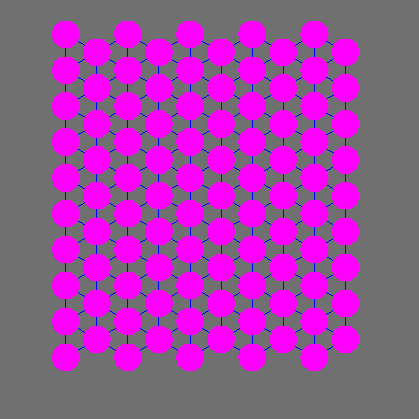
\includegraphics[width=6cm]{Images/hexagone.png}
\end{center}
\captionof{figure}{Image de la disposition des cellules à l'initialisation de la simulation.}

\subsection{Interactions entre cellules}

\subsubsection{Recherche des cellules adjacentes}

Pour commencer, toute cellule doit connaître toutes ses cellules adjacentes pour pouvoir interagir avec elles.\\
Pour cela nous avons utilisé un arbre KD pour optimiser la recherche des cellules. En effet l'arbre KD permet de réaliser une recherche des points inclus dans une sphère plus rapidement qu'une simple recherche linéaire.\\
Pour ce faire au début de chaque nouvelle étape compète de simulation, l'arbre KD est détruit puis remplacé par un nouveau vide. Ensuite, nous ajoutons toutes les positions des cellules dans l'ordre (en effet le numéro d'ajout et le seul moyen de retrouver la cellules par rapport à sa position) puis nous exécutons le tri des positions dans l'arbre KD.\\
Après avoir instancié l'arbre, chaque cellule peut rechercher ses cellules adjacentes dans un rayon égal à la norme d'un vecteur (1~; 1) (la distance originelle entre les cellules) puis enregistrer ces cellules dans une liste utilisé jusqu'à la re-création de l'arbre KD, donc du déplacement des cellules.

\begin{center}
  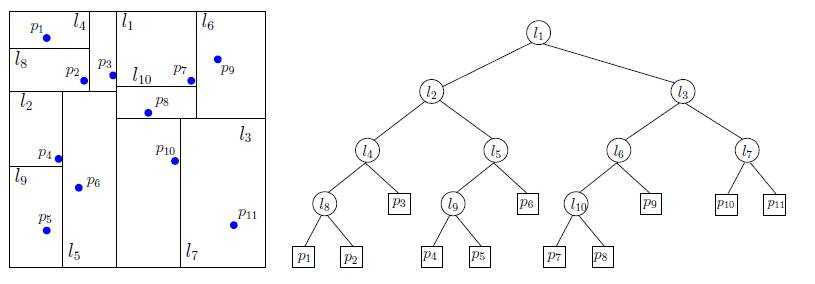
\includegraphics[width=12cm]{Images/kd_tree.jpg}
\end{center}
\captionof{figure}{Schéma d'un arbre KD en deux dimensions ainsi que sa hiérarchie.}


\subsubsection{Cellules en collisions}

Les cellules ne peuvent avoir d'interactions autre que la collision avec des cellules appartenant à une plaque tectonique différentes.\\
Prenons l'exemple de deux plaques qui se rencontrent, il y a alors une collision (puis subduction ou obduction dans certains cas).\\
Chaque cellule étant positionnée sur la surface de contact entre ces deux plaques est donc considérée en collision avec la cellule correspondante dans la plaque tectonique opposée.\\
Pour obtenir cette cellule en question, nous nous aidons de l'arbre KD qui nous donne une liste de cellules toutes adjacentes.\\
Dans cette liste nous ne retenons que les cellules ayant une plaque tectonique différente de celle de la cellule étudié.\\
Enfin ces cellules dites en collision n'interagiront qu'avec le centre instantané de rotation (décrit plus bas), laissant chacune de leur plaque tectonique respective déformer leurs cellules indépendamment.

\subsubsection{Propagation par front de cellules}

Pour propager la vélocité plusieurs méthodes ont été envisagé, la première entant la plus simple, se compose simplement d'une itération linéaire pour toutes les cellules existantes.\\
Ainsi chacune d'elle devra propager sa propre vélocité à ses cellules adjacentes.\\
Mais cette méthode est totalement erronée, car si nous faisons l'itération de toutes les autres cellules avant la cellule en collision, celle ci n'aura d'effet que sur ses seuls cellules adjacentes, et non sur toute la plaque.\\
Pour remédier à ce problème nous avons dû aborder une approche par fronts partant de la cellules en collision et s'étendant sur toute la plaque (formant ainsi une onde.\\
Deux méthodes s'offraient à nous :
\begin{itemize}
\item La première est de trouver toutes les cellules dans un intervalle de rayons par rapport à la cellule en collision ;
\item La deuxième méthode, récursive, consiste à créer un front d'origine avec seulement la cellules en collision et chaque front créé ainsi le suivant en ajoutant les cellules adjacentes n'ayant jamais participé au front.
\end{itemize}
Chacune de ces méthodes ont leurs avantages et inconvénients.\\
La première ne fonctionne que avec une plaque rectangulaire, en effet si la plaque est coudé les cellules de l'autre côté du coude seront déjà dans le front avant celles dans le coude, si la cellule en collision se trouve sur une des extrémités.\\
Ce problème n'est plus avec la deuxième méthode, mais celle ci a pour désavantage de ne pas former un front circulaire, mais basé sur la disposition des cellules, donnant ainsi un front hexagonal pour une disposition en nid-d'abeille.\\
Pesant le pour et le contre et en tenant compte du temps de calculs (notre implémentation d'arbre KD ne permettait pas une recherche par intervalle de rayons ce qui nous oblige à faire deux recherches par rayon et de supprimer le doublons) nous avons choisi la méthode récursive.\\
Pour ce faire les cellules possèdent maintenant deux nouvelles propriétés mutable~: une pour savoir si la cellule à déjà fait partie du front (cela signifie aussi que la cellule a déjà propagée sa vélocité) :\\ $a_C$ et l'autre pour savoir si la cellule fait actuellement partie du front : $b_C$.\\
Ces deux variables sont initialisées à faux au début de chaque étape complète de simulation.\\
Pour chaque cellules en collision nous créons un nouveau front ne contenant que celle ci, toutes les cellules contenus dans le front sont considérées comme déjà calculées et ne vont plus faire partie du front, donc elles voient $b_C$ et $a_C$ mis à vrai durant la propagation de vélocité sur leurs cellules adjacentes.\\
Ensuite chaque cellules dans le front itère sur toutes ses cellules adjacentes et les ajoute si leurs deux propriétés sont faussent (elle n'ont pas et ne font pas partie du front).\\
Chaque cellule remplissant ces conditions est alors ajoutée dans le front et vois $b_C$ mis a vrai car elle fait désormais partie du front.\\
Ainsi nous créons nouveau front grâce à l'ancien sans cellules en doublons.\\
Dès que le front ne contient plus aucune cellules, cela signifie que nous avons finit avec la cellule en collision actuelle et pouvons passer à la prochaine cellule en collision ou recommencer un étape complète de simulation. \\

\medbreak
\begin{algorithmic}[1]
   \STATE Création du front $F$.
   \FOR{$i_c$ de $0$ jusqu'à $(n_c - 1)$}
      \STATE Ajouter $C_{i_c}$ dans $F$.
      \STATE $b_{C_{i_c}} = Vrai$.
      
      \WHILE{$n_f > 0$}
      \FOR{$i_f$ de $0$ jusqu'à $(n_f - 1)$}
	\FOR{$i_a$ de $0$ jusqu'à $(n_a - 1)$}
	  \IF{non $a_{C_{i_a}}$ et non $b_{C_{i_a}}$}
	    \STATE Propagation de vélocité vers $C_{i_a}$.
	  \ENDIF
	\ENDFOR
	\STATE $a_{C_{i_f}} = Vrai$.
      \ENDFOR

      \FOR{$i_f$ de $0$ jusqu'à $(n_f - 1)$}
	\FOR{$i_a$ de $0$ jusqu'à $(n_a - 1)$}
	  \IF{non $a_{C_{i_a}}$ et non $b_{C_{i_a}}$}
	    \STATE Ajouter $C_{i_a}$ dans $F$.
	    \STATE $b_{C_{i_a}} = Vrai$.
	  \ENDIF
	\ENDFOR
      \ENDFOR
      \ENDWHILE
      \FOR{$i_t$ de $0$ jusqu'à $(n_t - 1)$}
	\STATE $a_{C_{i_t}} = Faux$.
	\STATE $a_{C_{i_t}} = Faux$.
      \ENDFOR
   \ENDFOR
\end{algorithmic}
\medbreak

Ou $n_t$ est le nombre de cellules total dans la simulation, $n_c$ le nombre de cellules en collision, $n_f$ nombre de cellules dans le front, $n_a$ nombre de cellules adjacentes à une cellule donnée, $a_C$ à vrai si la cellule a déjà fait partie du front donc à déjà propagée sa vélocité et $b_C$ à vrai si la cellule fait actuellement partie du front. \\

\begin{center}
  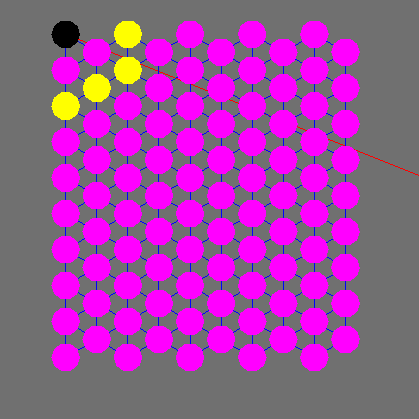
\includegraphics[width=4cm]{Images/front_1.png}
  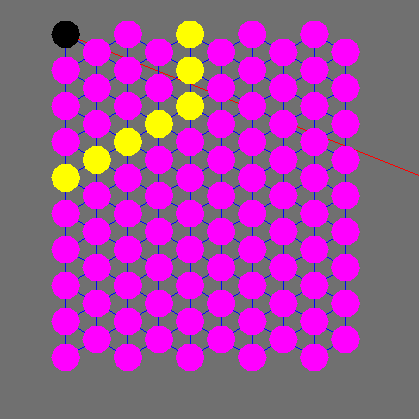
\includegraphics[width=4cm]{Images/front_2.png}
  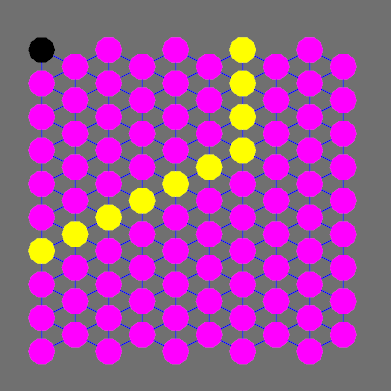
\includegraphics[width=4cm]{Images/front_3.png}
\end{center}
\begin{center}
  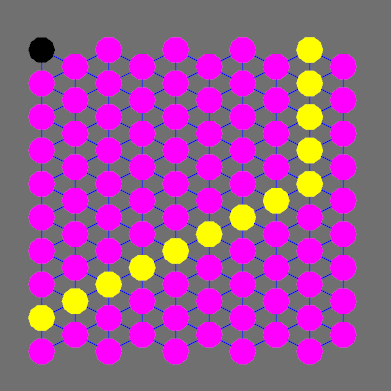
\includegraphics[width=4cm]{Images/front_4.png}
  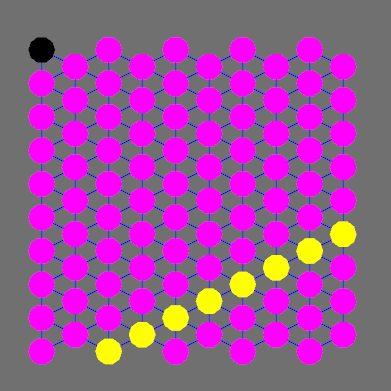
\includegraphics[width=4cm]{Images/front_5.png}
  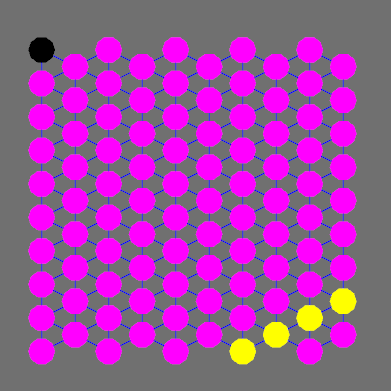
\includegraphics[width=4cm]{Images/front_6.png}
\end{center}
\captionof{figure}{Échantillons de six photos dans le temps montrant l'expansion du front aux cellules non calculées.
En noir la cellule en collision, en jaune les cellules du front et en violet les autres cellules.}

\subsubsection{Calques de vélocité}

Pour éviter des interférences entre les différentes propagations de vélocité des cellules en collision, nous utilisons des calques uniques contenant une vélocité par cellules, chacun de ces calques sont liés à une cellule en collision.
Au début de l'étape complète de simulation chaque cellule réserve dans ses variables une liste de vecteur pour chaque cellules en collision puis pour chaque propagation de vélocité des cellules en collision, les cellules affectées ne travaillent que sur le vecteur correspondant au numéro de la cellule en collision.
Puis à la fin de l'étape complète de simulation tous les vecteurs sont ajoutés entre eux pour donner le déplacement a appliquer à la cellule. \\

\begin{center}
  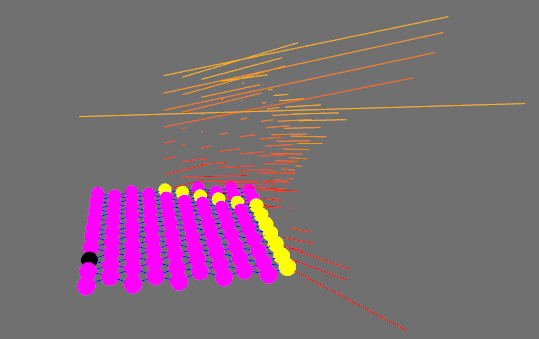
\includegraphics[width=8cm]{Images/calque.png}
\end{center}
\captionof{figure}{Photo de la représentation graphique des calques de vélocité, les premiers calques sont en rouge et les derniers en jaune. Nous pouvons observer pour chaque cellule sa vélocité calculée pour un calque particulier.}

\subsubsection{Centre instantané de rotation}

Comme nous l'avons expliqué, chaque cellule dans le front doit appliquer une vélocité aux cellules qui feront partie du front l'itération suivante.
Mais quelle doit être la direction de cette vélocité et sa norme~?\\
Prenant le cas de deux cellules $C_1$ et $C_2$.
$C_1$ fait partie du front et $C_2$ une de ses adjacentes non calculées, $C_1$ reçoit une vélocité $\vv{u}$, $C_2$ devra recevoir une vélocité $\vv{v}$ et $\vv{w}$ représente le vecteur de $C_1$ vers $C_2$.
L'estimation de la direction de la vélocité dans un modèle sans friction est des plus simple, elle équivaut au vecteur allant de la cellule $C_1$ vers $C_2$ : $\vv{w}$, mais l'estimation de la norme de ce vecteur est quant à elle bien plus compliquée.\\
La fonction calculant cette norme doit apporter les résultats suivants~:
lorsque le vecteur $\vv{w}$ est colinéaire à $\vv{u}$ (les deux cellules sont alignées sur la vélocité) la cellule $C_2$ doit recevoir toute la vélocité $\vv{v} = \vv{u}$ et, au contraire, si $\vv{w}$ et $\vv{u}$ forment un angle $\frac{\pi}{2}$ alors la cellule $C_2$ ne doit recevoir aucune vélocité, $\vv{v} = \vv{0}$, car elle et disposé latéralement à la cellule $C_1$ et n'étant pas dans un modèle avec friction, elle ne bouge pas.\\
La loi répondant à ces deux cas est le « Centre instantané de rotation d'un solide ».
Cette loi permet de mettre en relation la vélocité à deux points de contacts sur deux plan d'un solide grâce à une rotation.\\
Prenons l'exemple d'une échelle (le modèle est sans friction, sans gravité et uniquement sur un plan) posée avec un angle faible $\alpha$ sur un mur perpendiculaire au sol, elle forme deux points de contacts $P_1$ et $P_2$, $P_1$ en haut de l'échelle contre le mur et $P_2$ en bas de l'échelle contre le sol.
Si nous appuyons sur le haut de l'échelle dans le direction du mur celle-ci va avoir tendance à glisser en direction du sol.\\
En instantané nous pouvons faire l'approximation de ce mouvement par un rotation dont le centre serait l'intersection des deux droites perpendiculaires au sol et au mur passant respectivement par les points $P_1$ et $P_2$.\\
Nous nommerons $\vv{u}$ la vélocité de l'échelle à $P_1$, $\vv{v}$ la vélocité à $P_2$ lors du glissement, $C$ le centre de rotation, $d$ la distance entre $C$ et $P_1$, $f$ la distance entre $C$ et $P_2$ et enfin $\alpha$ l'angle de rotation.

\begin{center}
\begin{tikzpicture}[line cap=round,line join=round,>=triangle 45,x=0.8cm,y=0.8cm]
\clip(-2,-1) rectangle (8,8);
\draw [shift={(4,7)},color=qqwuqq,fill=qqwuqq,fill opacity=0.1] (0,0) -- (180:1.87) arc (180:194.04:1.87) -- cycle;
\draw [shift={(4,7)},color=qqwuqq,fill=qqwuqq,fill opacity=0.1] (0,0) -- (-90:1.97) arc (-90:-74.21:1.97) -- cycle;
\draw (0,6)-- (4,7);
\draw [domain=-2:8] plot(\x,{(-0-0*\x)/4});
\draw [->] (0,7) -- (0,6);
\draw (0,-2) -- (0,8);
\draw (0,7)-- (4,7);
\draw (4,7)-- (4,0);
\draw (4,7)-- (5.98,0);
\draw [->] (4,0) -- (5.98,0);
\draw [->] (0,7) -- (4,0);
\begin{scriptsize}
\fill [color=xdxdff] (4,7) circle (1.5pt);
\draw[color=xdxdff] (4.16,7.24) node {$C$};
\fill [color=xdxdff] (4,0) circle (1.5pt);
\draw[color=xdxdff] (4.16,0.25) node {$B$};
\draw[color=black] (0.14,6.63) node {$u$};
\draw[color=black] (2.07,6.84) node {$d$};
\draw[color=black] (3.72,3.64) node {$f$};
\draw[color=qqwuqq] (3.21,6.91) node {$\alpha$};
\draw[color=black] (5.04,0.21) node {$v$};
\draw[color=qqwuqq] (4.41,5.89) node {$\beta$};
\draw[color=black] (2.13,3.66) node {$w$};
\end{scriptsize}
\end{tikzpicture}
\end{center}
\captionof{figure}{Ci dessus le schéma représentant la mise en situation du CIR avec l'exemple de l'échelle.}
\bigbreak

Cette rotation nous permet de lier la norme de la vélocité appliquée sur le haut de l'échelle $\vv{u}$ et celle du glissement $\vv{v}$ grâce à $\alpha$, $d$ et $f$. \\
\begin{center}
  $||\vv{u}|| = d \times \alpha$ \medbreak
  $||\vv{v}|| = f \times \alpha$
\end{center}
Dans le cas de nos deux cellules $C_1$ et $C_2$ en compression, nous ne connaissons pas $\alpha$ ni le centre $C$ donc $d$ et $f$ de même.
Nous nommerons $\beta$ l'angle obtenu entre $\vv{u}$ et $\vv{w}$.
Cette angle nous permet de calculer les deux distances $d$ et $f$~:
\begin{center}
  $\displaystyle{d = \frac{||\vv{w}||}{\sin{\beta}}}$ \medbreak
  $\displaystyle{f = \frac{||\vv{w}||}{\tan{\beta}}}$
\end{center}
Puis $\alpha$ est déduit de $d$ et de la norme de $\vv{u}$~:
\begin{center}
  $\displaystyle{\alpha = \frac{||\vv{u}||}{d}}$
\end{center}
La formule complète pour calculer la norme de $\vv{v}$ se présente~:
\begin{center}
  \boxed{\displaystyle{||\vv{v}|| = \frac{||\vv{w}|| \times ||\vv{u}||}{\tan{\beta} \times d}}}
\end{center}
L'implémentation de cette loi doit traiter quelques cas particuliers pour éviter toutes divisions par zéro, si $\cos\beta = 0$ alors $\vv{v} = \vv{0}$ et si $\sin\beta = 0$ alors $\vv{v} = \vv{u}$.

\begin{center}
\begin{tikzpicture}[line cap=round,line join=round,>=triangle 45,x=0.4cm,y=0.4cm]
\clip(-5,-5) rectangle (17,12);
\draw [shift={(16.25,7)},color=qqwuqq,fill=qqwuqq,fill opacity=0.1] (0,0) -- (-150.26:4.15) arc (-150.26:-139.13:4.15) -- cycle;
\draw [shift={(16.25,7)},color=qqwuqq,fill=qqwuqq,fill opacity=0.1] (0,0) -- (180:4.15) arc (180:191.31:4.15) -- cycle;
\draw[color=qqwuqq,fill=qqwuqq,fill opacity=0.1] (0.88,7) -- (0.88,7.88) -- (0,7.88) -- (0,7) -- cycle; 
\draw[color=qqwuqq,fill=qqwuqq,fill opacity=0.1] (4.76,0.44) -- (4.33,1.2) -- (3.56,0.76) -- (4,0) -- cycle; 
\draw (0,-2) -- (0,12);
\draw [domain=-4:16] plot(\x,{(-0-0*\x)/4});
\draw [->] (0,7) -- (0,3.75);
\draw(0,7) circle (2cm);
\draw(4,0) circle (2cm);
\draw [domain=-4:16] plot(\x,{(--28-7*\x)/4});
\draw [->] (4,0) -- (5.38,-2.41);
\draw (0,7)-- (16.25,7);
\draw (16.25,7)-- (4,0);
\draw (5.38,-2.41)-- (16.25,7);
\draw (0,3.75)-- (16.25,7);
\draw [->] (0,7) -- (4,0);
\begin{scriptsize}
\draw[color=black] (0.27,5.65) node {$u$};
\draw[color=black] (4.92,-0.84) node {$v$};
\fill [color=uququq] (16.25,7) circle (1.5pt);
\draw[color=uququq] (16.59,7.53) node {$C$};
\draw[color=black] (8.28,6.67) node {$d$};
\draw[color=black] (9.86,4.32) node {$f$};
\draw[color=qqwuqq] (14.76,5.69) node {$\beta$};
\draw[color=qqwuqq] (14.47,6.86) node {$\alpha$};
\draw[color=black] (2.26,3.85) node {$w$};
\end{scriptsize}
\end{tikzpicture}
\captionof{figure}{Représentation du CIR au niveau des cellules.}
\end{center}
\bigbreak

Cette formule convient parfaitement pour une interaction avec une seule cellule, mais dans la plupart des cas il y en a plus. En effet au début de la simulation une cellule du front peut avoir au maximum quatre cellules adjacentes non calculées.
Nous ne pouvons alors pas utiliser la même formule car la somme de la norme des vélocités appliquées aux cellules pourrait être supérieur à $||\vv{u}||$, cela signifierait une création de vélocité.
Pour palier à ce problème toutes les vélocités sont divisées par le nombre de cellules adjacentes non calculées.

\begin{center}
  $\displaystyle{\sum \limits_{i=1}^n ||\vv{v}_{max}|| = ||\vv{u}||}$ \medbreak
  $\displaystyle{||\vv{v}_{max}|| = \frac{||\vv{u}||}{n}}$
\end{center}

Ou $n$ le nombre de cellules adjacentes non calculées.

\begin{center}
  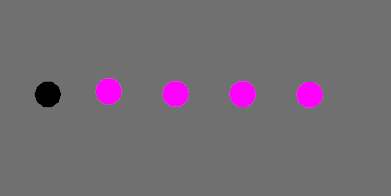
\includegraphics[width=4cm]{Images/cir_1.png}
  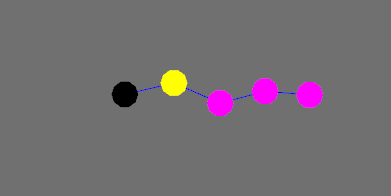
\includegraphics[width=4cm]{Images/cir_2.png}
  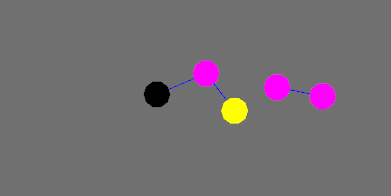
\includegraphics[width=4cm]{Images/cir_3.png}
  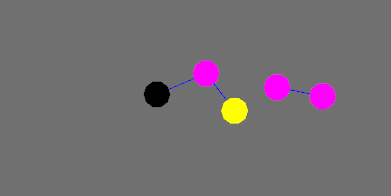
\includegraphics[width=4cm]{Images/cir_3.png}
  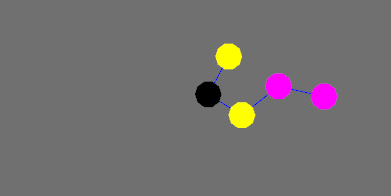
\includegraphics[width=4cm]{Images/cir_4.png}
  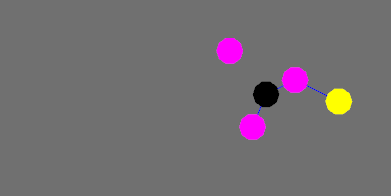
\includegraphics[width=4cm]{Images/cir_5.png}    
\end{center}
\captionof{figure}{Échantillons dans le temps de six images montrant l'utilité du Centre instantané de rotation.
Les cellules sont disposées avec un léger aléatoire lors de leur création.
Ainsi nous évitons un cas trop « parfait ».}

\subsubsection{Compression et traction entre cellules}

\paragraph{Loi de Hooke}
\medbreak
Maintenant que nous avons la formule pour la répartition de la vélocité entre les cellules, nous devons gérer les cas de compression et de traction.
Les cellules adjacentes doivent toujours viser une distance parfaite équivalente à $1$.
En théorie, la compression et la traction doivent être régies par la loi de Hooke complémentée du module de Young. Cette loi met en relation le coefficient de déformation (en \%), la contrainte appliquée sur le matériau (en Pa) et la caractéristique du matériau trouvé dans le module de Young (en Pa).
La formule de cette loi se présente sous la forme de~:
\begin{center}
  \boxed{\sigma = E \times \epsilon}
\end{center}
Où $\sigma$ est la contrainte appliquée sur le matériau, $E$ la valeur du module de Young pour ce matériau et $\epsilon$ le coefficient de déformation. \\
Le module de Young contient de nombreuses valeur de $E$ pour la majorité des matériaux, dans notre cas nous ne voulons que les valeurs des roches ci dessous~:
\begin{itemize}
  \item calcaire : 20 à 70 GPa ;
  \item granite : 60 GPa.
\end{itemize}


<<<<<<< HEAD
\paragraph{Approximation du comportement de la compression et traction.}

Cette formule nécessite de connaître la contrainte entre les deux cellules, or notre modèle de simulation se base uniquement sur la vélocité des cellules.\\
Nous devons donc utiliser une approximation, premièrement il faut définir le comportement de cette approximation.\\
Quand la distance entre deux cellules est supérieur à $1$ nous sommes en traction et nous devons alors ajouter une vélocité opposée à au vecteur entre les deux cellules.\\
Sinon si la distance est inférieur à $1$, nous devons ajouter une vélocité colinéaire au vecteur entre les deux cellules pour la compression.\\
Pour augmenter la norme de la vélocité, une fonction carré convient parfaitement et peut aussi être multipliée par un facteur pour être plus accentué, mais cette fonction ne traite que de la compression car elle est toujours positive.\\
=======
\paragraph{Approximation du comportement de la compression et traction}
\medbreak
Cette formule nécessite de connaître la contrainte entre les deux cellules, or notre modèle de simulation se base uniquement sur la vélocité des cellules.
Nous devons donc utiliser une approximation, premièrement il faut définir le comportement de cette approximation.
Quand la distance entre deux cellules est supérieur à $1$ nous sommes en traction et nous devons alors ajouter une vélocité opposée à au vecteur entre les deux cellules.
Sinon si la distance est inférieur à $1$, nous devons ajouter une vélocité colinéaire au vecteur entre les deux cellules pour la compression.
Pour augmenter la norme de la vélocité, une fonction carré convient parfaitement et peut aussi être multipliée par un facteur pour être plus accentué, mais cette fonction ne traite que de la compression car elle est toujours positive.
>>>>>>> fee67899dfe2d18926750a6492e39b3d0f8ca9d2
Nous devons donc utiliser l'opposé d'un carré quand $x$ est négatif.
\medbreak
\begin{center}
  Si traction : $d' \leqslant 0 \Rightarrow E = -d'^2$ \medbreak
  Si compression : $d' > 0 \Rightarrow E = d'^2$
\end{center}
Où $d'$ est la différence entre la distance voulu $1$ et la distance entre les deux cellules. \\

\begin{center}
  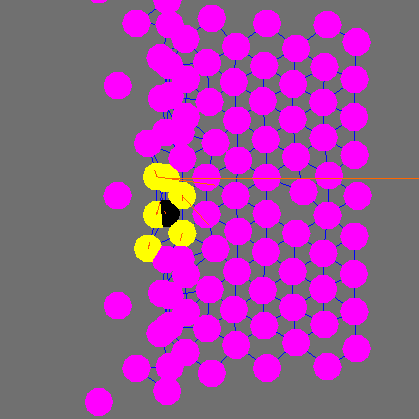
\includegraphics[width=5cm]{Images/normal_1.png}
  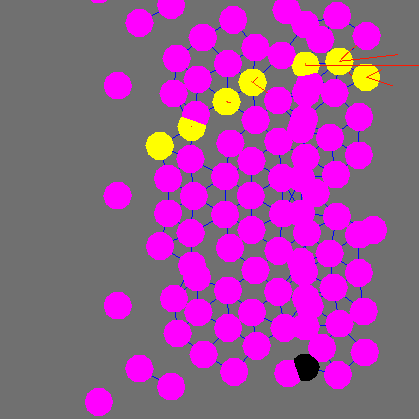
\includegraphics[width=5cm]{Images/normal_2.png}
\end{center}
\captionof{figure}{Deux échantillons de simulation sans compression, les cellules en collisions (en noir) rentrent dans la plaque.}
\begin{center}
  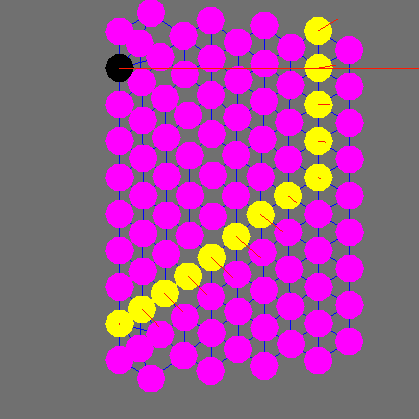
\includegraphics[width=5cm]{Images/compression_1.png}
  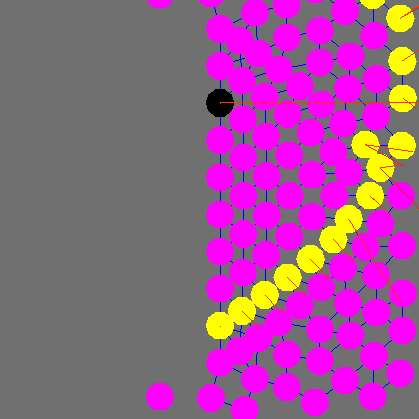
\includegraphics[width=5cm]{Images/compression_2.png}
\end{center}
\captionof{figure}{Deux échantillons de simulation avec compression, les cellules en collisions (en noir) poussent d'abord toutes les autres cellules après elles.} 

\subsubsection{Friction entre cellules}
Les cellules doivent exercer entre elles une friction pour éviter de glisser.\\
Notre modèle actuel se rapproche plus d'un ensemble de billes, où chaque billes essaierait de maintenir une distance égale entre ses billes adjacentes (cohésion de la roche).
Si cette équidistance devait casser, les relations entre ces billes devraient êtres supprimées (si la roche se fissure).\\
Cette situation est désirée lors d'une fissure dans une plaque tectonique (tous les liens inter-cellulaire se cassent le long de la faille), mais désavantageux dans une simple simulation de compression par un front de collision, car celle ci ressemblera tout simplement à un simulation de grains de sables.\\
La friction est alors utilisée ici comme une force correctrice du centre instantané de rotation, car en effet la traction ne peut compenser une faible valeur calculée avec le CIR.\\
La plus simple des lois à mettre en place pour la friction est la loi de Coulomb. \\
Cette loi nous donne deux états~: en friction ou en détachement (glissement), libre à nous de mettre les bons facteurs (inférieur à 1) derrière ces deux états.\\
Pour trouver dans quelle état deux cellules $C_1$ et $C_2$ se trouvent nous devons appliquer la formule suivante~:
\begin{center}
  \boxed{T_0 = f_0 \times N}
\end{center}
\bigbreak
Où $N$ est la pression entre $C_1$ et $C_2$, $T$ la force tangentielle entre $C_1$ et $C_2$, $T_0$ la force maximale pour être en situation de friction, $f_0$ la valeur du coefficient de friction.
\medbreak
Si $T > T_0$ : détachement.
Si $T \leqslant T_0$ : friction.
\medbreak
Cette loi peut être représentée par un cône de friction pour simplifier celle-ci~: \\

\begin{center}
  \begin{tikzpicture}[line cap=round,line join=round,>=triangle 45,x=0.8cm,y=1.0cm]
    \clip(-4,-2) rectangle (4,2);
    \draw [shift={(0,0)},color=qqwuqq,fill=qqwuqq,fill opacity=0.1] (0,0) -- (53.13:0.63) arc (53.13:126.87:0.63) -- cycle;
    \draw (-1.5,2)-- (0,0);
    \draw (0,0)-- (1.5,2);
    \draw (1.5,2)-- (-1.5,2);
    \draw [domain=-4:4] plot(\x,{(-0-0*\x)/4});
    \draw (0,0)-- (0,1.41);
    \draw (-1.06,1.41)-- (1.06,1.41);
    \begin{scriptsize}
      \draw[color=qqwuqq] (0.06,0.4) node {$f_0$};
      \draw[color=black] (0.21,0.79) node {$N$};
      \draw[color=black] (0.03,1.33) node {$T$};
    \end{scriptsize}
  \end{tikzpicture}
\end{center}

Malheureusement comme notre modèle de simulation est essentiellement cinématique (se basse essentiellement sur la vélocité), nous ne pouvons donc pas fournir une force et alors utiliser la loi de Coulomb.
Cette loi restera inutilisé dans la simulation, mais nous savons qu'à un moment donné nous en auront besoin.
De plus, toutes les cellules auront besoin d'une pression par défaut~: en effet si il n'y a pas de pression $N = 0$ et $T_0 = 0$.
Pour éviter ce problème nous pourrons spécifier une pression par défaut entre les cellules à l'initialisation de la simulation, mais cela signifiera que deux cellules ne se repousseront pas même si il y a une pression entre elles. 

\subsection{Les limites de la simulation}

Notre objectif initial était de simuler la géomorphologie des alpes sur une parcelle de 100km de côté et de 10km de profondeur.
Si nous gardons comme taille 10m par cellules, la simulation se porte alors à~:
\begin{center}
  $100 \times 10^2 \times 100 \times 10^2 \times 10 \times 10^2 = 1 \times 10^{11}$ cellules
\end{center}
Nous devons donc utiliser 10 milliards de cellule pour simuler les alpes.
Nous allons voir plus bas que notre objectif initial était loin d'être réalisable.

\subsubsection{Les limites du réalisme}

Comme nous l'avons de nombreuses fois montré, notre simulation a été obligé d'utiliser plusieurs approximations.
La répartition de la vélocité n'est pas exacte et nous utilisons pas la loi de Hooke pour la compression à cause du modèle choisi.
L'ensemble forme ainsi une pile d'approximation n'est sans moins marchant superbement en cohésion.
Tout le long de la création de la simulation nous avions remarqué de nombreuses instabilité, certaine fois des « explosions de cellules », celle ci était alors éjecté de la plaque à une très grande distance et vitesse.
Cela prouve que la simulation géomorphologique n'est pas une mince à faire pour avoir un résultat un tant soit peu réaliste.

\subsubsection{Les limites de temps de calcul}

\begin{center}
  \begin{tikzpicture}
    \begin{axis}[height=10cm,width=10cm, axis x line=bottom, axis y line=left, grid=major, xlabel={Nombre de cellules}, ylabel={Temps de calcul (en ms)}, title={Temps de calcule (en ms) en fonction du nombre de cellules pour une cellule en collision.}]
      \addplot coordinates {
	(100,2.5)
	(2500,41)
	(10000,167)
	(22500,366)
	(40000,654)
	(62500,1010)
	(90000,1466)
      };
    \end{axis}
  \end{tikzpicture}
\end{center}

Comme nous pouvons le voir la complexité asymptotique (la relation entre le nombre d'opération, donc implicitement du temps, et le nombre d'éléments dans un algorithme) est linéaire~: $O(n)$.
Donc pour une cellule le temps de calcul moyen est d'environ $0.01629$ ms/cellule, ainsi nous pouvons estimer que nos 10 milliards de cellules prendrons $16289999999$ms, ce qui fait 4525 heures et environs 189 jours.
Or nous n'avons pas qu'un cellule en collision, nous avons tout un côté de la plaque en collision soit $10000$ cellules en collision.
Cela augmente considérablement le temps de calcule pour arriver à 1890000 jours soit 5178 ans.
Il faut donc 5178 ans de calcul avant de voir une seule cellule bouger.
Nous pouvons en venir à la question suivante : simuler la géomorphologie numériquement ne serait il pas aussi long que d'observer ces phénomènes géomorphologiques.

\section{Conclusion}

Ce TPE aura été pour nous l'occasion de nous réunir sur un projet commun qui, en connectant nos différents centres d’intérêts, nous aura appris beaucoup de nouvelles choses en ce qui concerne la géologie, la géomorphologie et l'histoire des roches et la terre en général. \\
De plus, la recherche puis la création de notre simulateur fut un véritable défi technique, nous poussant à nous renseigner sur des domaines relativement pointus tant dans les mathématiques que dans la programmation informatique, afin d'offrir un démonstrateur certes incomplet, mais cependant fonctionnel et déjà assez intéressant. \\
Nous aurons énormément appris en géologie et de ce point de vue le TPE aura été une réussite. \\
Même si notre simulateur n'est pas encore capable de simuler des comportements complexes, il apparaît qu'il possède en lui les germes d'un moteur plus performant, c'est pourquoi l'affaire reste à suivre. \\ De plus,pouvons déjà simuler un environnement réduit en deux dimensions, ce qui reste intéressant pour les fluides visqueux par exemple. Nous somme heureux d'être arrivé à un résultat dans notre travail mutuel et remercions nos accompagnateurs pour leurs critiques constructives.

\end{document}
